\subsubsection{WEP}

The \gls{wep} algorithm is part of the original \gls{ieee} 802.11 standard and was intended to avoid eavesdropping and ensure privacy for those connected to a wireless network \cite{ieee_80211_2020}.

It relies on a secret that is known by the station and has been delivered to the wireless client, presumably via a secure channel, to accept or decline the authentication request. An encrypted challenge is sent to the client, which decrypts it using the shared key and sends the decrypted challenge back to the station, proving that it knows the password, thus should be authenticated successfully.

\paragraph{Algorithm}

\begin{figure}[h]
    \centering
    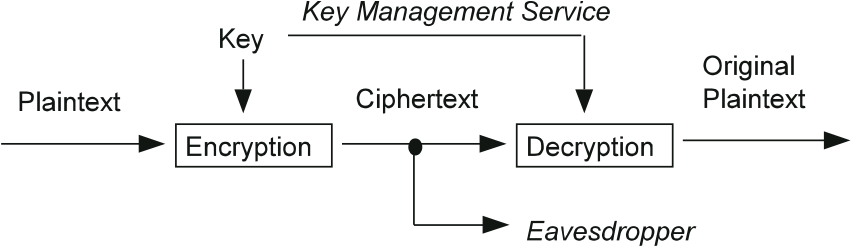
\includegraphics[width=\linewidth]{contents/background-in-wireless-networks/protected-network-standards/wep/algorithm/a-confidential-data-channel.png}
    \caption{A Confidential Data Channel}
    {Source: \cite{ieee_80211_2020}}
    \label{figure:ieee80211_figure43}
\end{figure}

The algorithm \cite{ieee_80211_2020} uses a key sequence produced by a \gls{prng} to encrypt and decrypt data, establishing a secure channel as shown in Figure \ref{figure:ieee80211_figure43}. The \gls{prng} used by \gls{wep} requires a 64-bit or 128-bit seed to initialize its initial state and derive the associated keystream. The \gls{wep} \gls{sk}, either 40 bits (\gls{wep}-40) or 104 bits (\gls{wep}-104) in size, and the \gls{iv}, 24 bits long, are concatenated and used as the seed for the \gls{prng}. The \gls{iv} content is random and its role is to avoid the \gls{prng} to be initialized with the same seed more than once, preventing the data from being encrypted with an already known key sequence.

The \gls{ia} is used to detect if the message sent via the wireless network was corrupted and possibly tempered with on transport, it takes the plaintext as input and produces 32 bits as the \gls{icv}.

\begin{figure}[h]
    \centering
    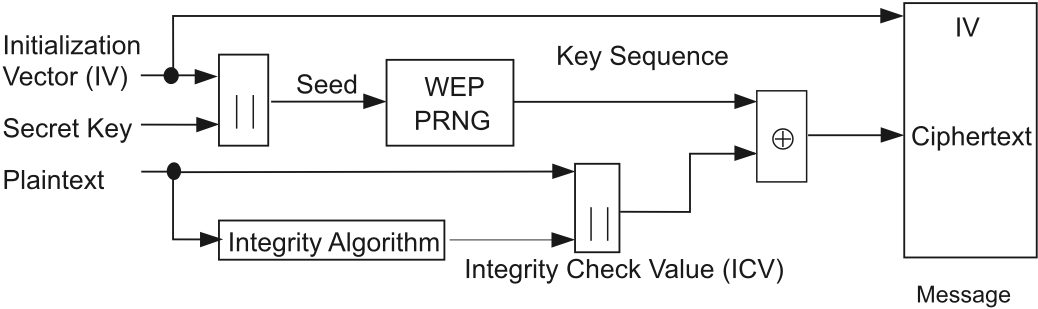
\includegraphics[width=\linewidth]{contents/background-in-wireless-networks/protected-network-standards/wep/algorithm/wep-encipherment-block-diagram.png}
    \caption{\gls{wep} Encipherment Block Diagram}
    {Source: \cite{ieee_80211_2020}}
    \label{figure:ieee80211_figure44}
\end{figure}

As illustrated on Figure \ref{figure:ieee80211_figure44}, to encrypt a message, the algorithm requires the \gls{sk}, the \gls{iv}, and the plaintext. First, the \gls{sk} and the \gls{iv} are fed to the \gls{prng}, and \gls{N} bits from the keystream are stored in \gls{KS}, where \gls{N} is the length of the plaintext added by the size of the \gls{icv}. Then the plaintext is fed to the \gls{ia} and the output is stored in \gls{icv}. The plaintext is concatenated with the \gls{icv} and XORed with \gls{KS}, resulting in the ciphertext. Finally, the \gls{iv} is concatenated with the ciphertext and returned as the output of the algorithm, the \gls{mpdu}.

\begin{figure}[h]
    \centering
    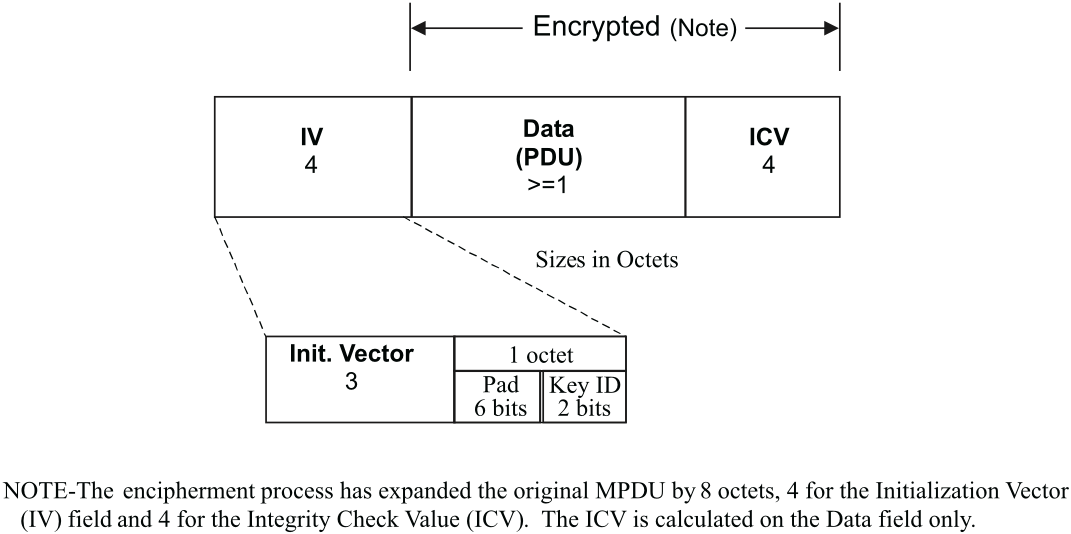
\includegraphics[width=\linewidth]{contents/background-in-wireless-networks/protected-network-standards/wep/algorithm/construction-of-expanded-wep-mpdu.png}
    \caption{Construction of Expanded \gls{wep} \gls{mpdu}}
    {Source: \cite{ieee_80211_2020}}
    \label{figure:ieee80211_figure46}
\end{figure}

Figure \ref{figure:ieee80211_figure46} shows the encrypted \gls{mpdu} as constructed by the \gls{wep} algorithm. It is transmitted over the wireless connection and then decrypted by the receiver. To decrypt the \gls{mpdu}, only the \gls{sk} is required. So the confidentiality of the data channel established using \gls{wep} essentially relies on the secrecy of the shared key.

\begin{figure}[h]
    \centering
    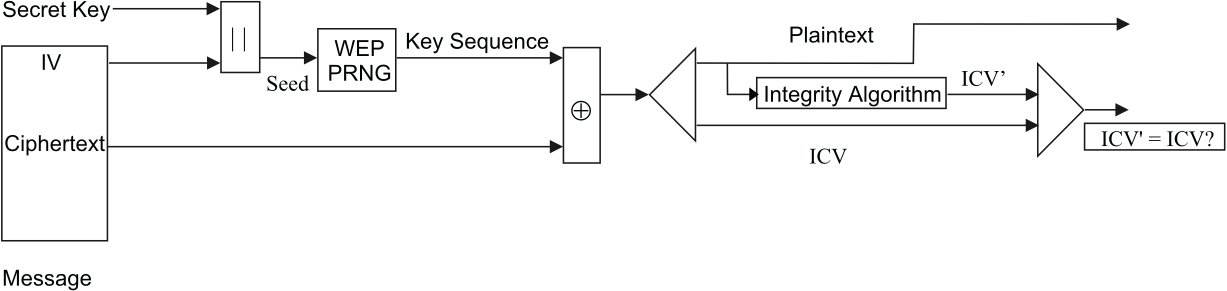
\includegraphics[width=\linewidth]{contents/background-in-wireless-networks/protected-network-standards/wep/algorithm/wep-decipherment-block-diagram.png}
    \caption{\gls{wep} Decipherment Block Diagram}
    {Source: \cite{ieee_80211_2020}}
    \label{figure:ieee80211_figure45}
\end{figure}

The decryption algorithm, as represented by Figure \ref{figure:ieee80211_figure45}, receives the \gls{sk} and the \gls{mpdu} to be decrypted. First, the \gls{iv} is extracted from the first 24 bytes of the \gls{mpdu} and appended to the \gls{sk}, resulting in the seed for the \gls{prng}. Then \gls{N} bits are consumed from the keystream and stored in \gls{KS}, \gls{N} is the length of the ciphertext and \gls{sk} the key sequence produced. The ciphertext is XORed with \gls{KS}, recovering the plaintext concatenated with the \gls{icv}. Finally, the plaintext is fed to the \gls{ia}, calculating \gls{icv}’. If the values of the extracted \gls{icv} and \gls{icv}’ are the same, the plaintext is successfully returned as the output of the algorithm. Otherwise, the \gls{mpdu} was corrupted and an error is sent to the \gls{mac} management.

\FloatBarrier

\paragraph{Security}

A compromise was made on the \gls{tkip} design to make possible its use on legacy \gls{wep} hardware. The forgery attacks were mitigated with the introduction of the Michael algorithm, but, due to computing power constraints, while blocking the forged packets it would cause a denial of service on the network \cite{ieee_80211_2020}.

As \gls{tkip} just encapsulates the \gls{wep} algorithm, it still relies on the security of the \gls{rc4} \gls{prng}. It was found that the keystream generated by \gls{rc4} is biased towards certain sequences and it made practical attacks against \gls{wpa}-\gls{tkip} networks within an hour \cite{rc4nomore}. The attacker would establish a \gls{tcp} connection with some victim on the network and would repeatedly send identical packets particularly sized with a well-known content over the connection. Then the wireless traffic was captured and filtered to only what would likely be an attacker's packet. Ciphertext statistics were extracted and plaintext likelihoods calculated using a combination of the \gls{fm} and \gls{absab} biases. Finally, the \gls{mic} key is derived from one of the candidates with the correct \gls{icv}, allowing any other packet of the victim to be fully decrypted.

